% 第9章：宇宙学
\section{宇宙学}
\label{sec:cosmology}

\subsection{引言：宇宙的演化图景}

CTUFT宇宙学从单一几何原理推导宇宙演化：
\begin{itemize}
    \item \textbf{暴涨}：来自谱维从10D到4D的过渡
    \item \textbf{暗能量}：$\Lambda$的几何起源
    \item \textbf{暗物质}：原初黑洞遗迹
    \item \textbf{重子生成}：CP破坏的几何来源
\end{itemize}

\subsection{扭转驱动暴涨}

\subsubsection{暴涨的几何机制}

在CTUFT中，暴涨不是由假设的暴胀子驱动，而是由谱维的维度转变驱动。

\begin{insight}[暴涨作为维度转变]
早期宇宙的高能状态对应谱维 $d_s \approx 10$。当宇宙膨胀和冷却时，谱维通过扭转场动力学"冻结"到 $d_s = 4$。这个过渡表现为指数膨胀——暴涨。
\end{insight}

\subsubsection{暴涨场作为谱维}

有效暴涨场是谱维偏离其低能值：
\begin{equation}
    \phi_{\text{inf}}(t) \equiv d_s(t) - 4
\end{equation}

动力学由扭转场能量密度驱动：
\begin{equation}
    \rho_{\text{inf}} = \rho_\tau = \frac{\tau_0^2}{\kappa^2} \cdot f(d_s)
\end{equation}

\subsubsection{慢滚参数}

慢滚参数可以从谱维流推导：
\begin{equation}
    \epsilon = -\frac{\dot{H}}{H^2} = \frac{3\tau_0^2}{2(d_s - 4)^2}
\end{equation}

当 $d_s \to 4$（接近维度冻结），$\epsilon \to \infty$，慢滚结束。

\subsection{早期宇宙中的谱维演化}

\subsubsection{维度转变动力学}

谱维从 $d_s = 10$ 到 $d_s = 4$ 的转变遵循：
\begin{equation}
    d_s(T) = 4 + \frac{6}{1 + (T/T_c)^2}
\end{equation}

其中 $T_c \sim 10^{16}$ GeV 是GUT能标。

\begin{figure}[htbp]
\centering
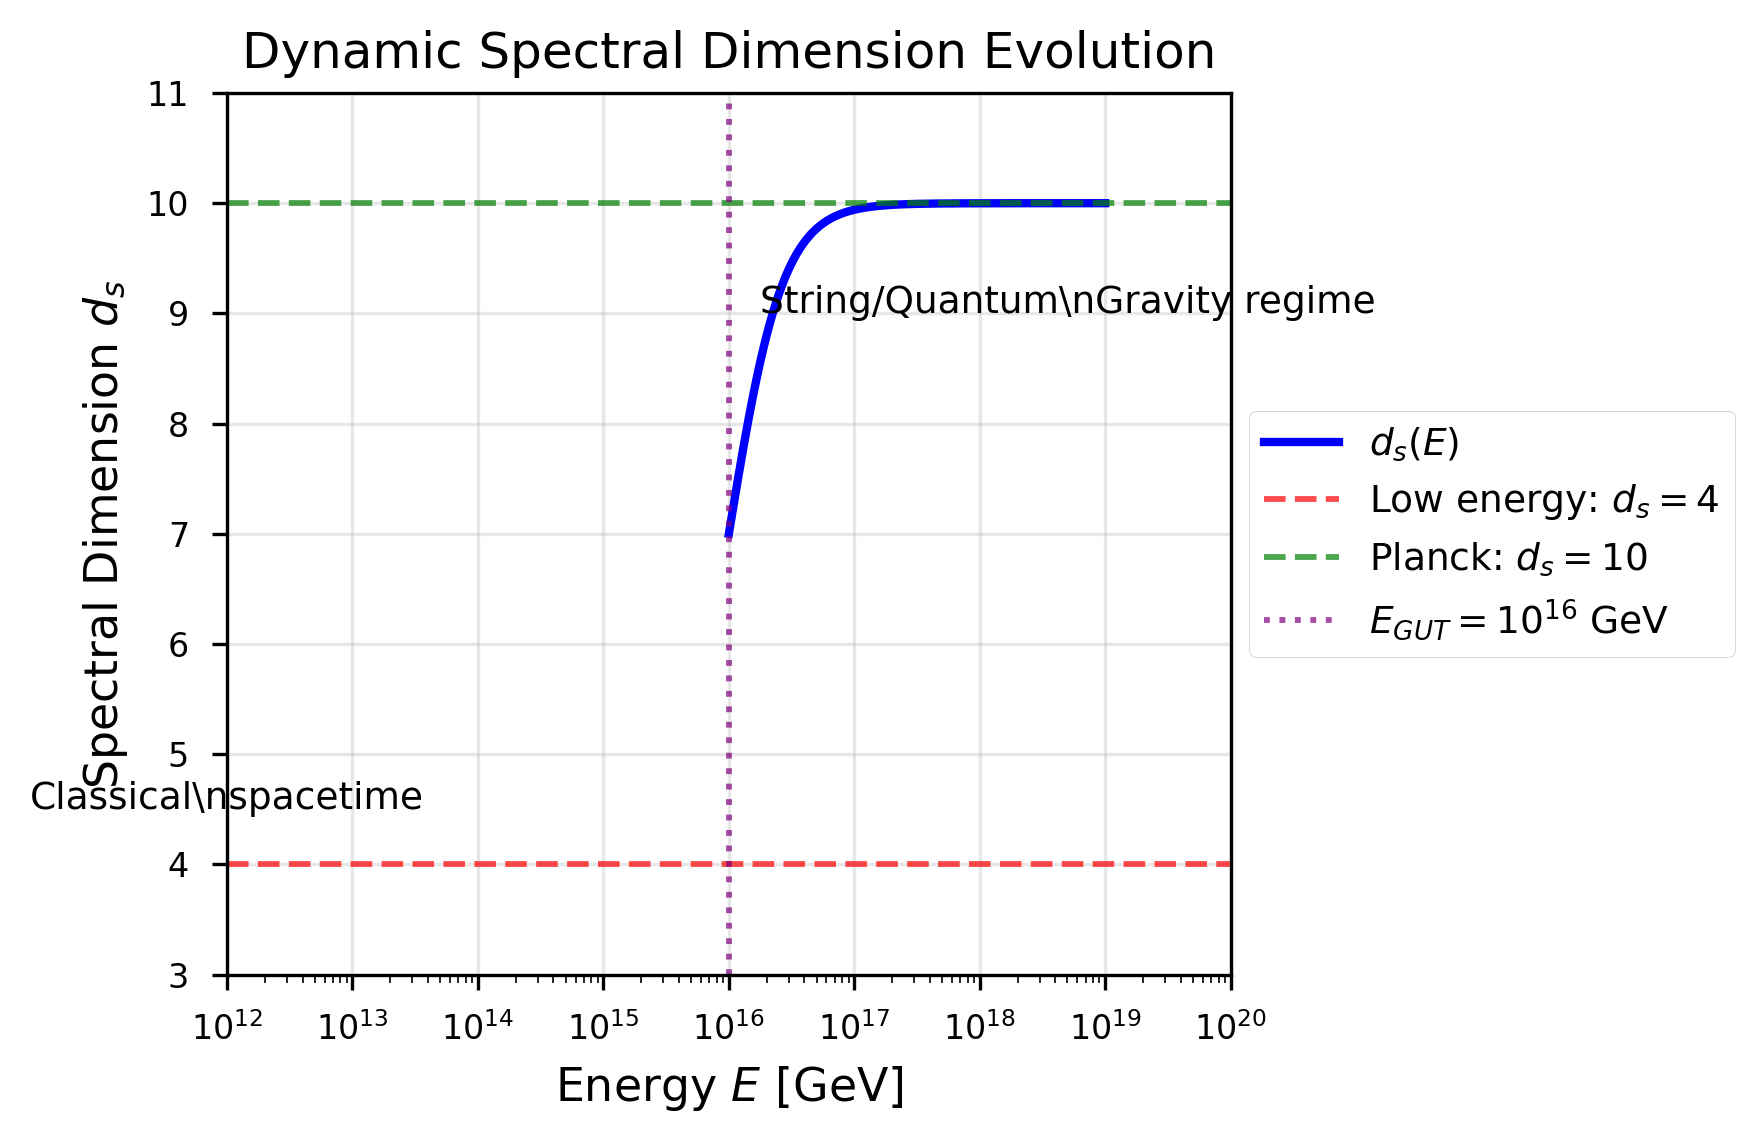
\includegraphics[width=0.8\textwidth]{figures/fig1_spectral_dimension.png}
\caption{宇宙演化中谱维的转变。在高能（$T \gg T_c$），$d_s \approx 10$。当 $T \sim T_c$，维度冻结到 $d_s = 4$。}
\label{fig:cosmic_spectral}
\end{figure}

\subsubsection{与热历史的关系}

维度转变与宇宙热历史的关系：
\begin{itemize}
    \item $T > T_c$：$d_s \approx 10$，统一力相
    \item $T \sim T_c$：暴涨，谱维冻结开始
    \item $T \ll T_c$：$d_s = 4$，标准4D宇宙学
\end{itemize}

\subsection{原初黑洞形成}

\subsubsection{形成机制}

在维度转变期间，密度涨落可能坍缩形成原初黑洞：
\begin{equation}
    \beta(M) = \frac{\rho_{PBH}(M)}{\rho_{\text{total}}} \sim \sigma^2 \cdot \exp\left(-\frac{\delta_c^2}{2\sigma^2}\right)
\end{equation}

其中$\sigma$是原初功率谱的振幅，$\delta_c \sim 0.45$是临界过密度。

\subsubsection{质量谱}

CTUFT预言原初黑洞的质量谱：
\begin{equation}
    \frac{dn}{dM} \propto M^{-5/2} \cdot f(\tau_0)
\end{equation}

峰值质量取决于转变时间尺度。

\subsection{暗物质：原初黑洞遗迹}

\subsubsection{量子遗迹作为暗物质}

原初黑洞蒸发后留下稳定的量子遗迹：
\begin{equation}
    M_{rem} \sim M_P \cdot \tau_0^{1/3} \sim 10^{-8} \text{ kg}
\end{equation}

这些遗迹作为暗物质候选者：
\begin{itemize}
    \item 冷暗物质：非相对论性
    \item 碰撞less：只有引力相互作用
    \item 稳定：扭转饱和阻止进一步蒸发
\end{itemize}

\subsubsection{丰度估计}

遗迹的暗物质丰度：
\begin{equation}
    \Omega_{\text{rem}} \sim 10^{-8} \cdot f_{\text{PBH}} \cdot \Omega_{\text{DM}}
\end{equation}

如果原初黑洞在早期宇宙中丰富形成，它们可能构成暗物质的显著部分。

\subsection{暗能量：$\Lambda$的几何起源}

\subsubsection{宇宙学常数问题}

标准宇宙学中，观测到的暗能量密度：
\begin{equation}
    \rho_\Lambda^{obs} \sim 10^{-47} \text{ GeV}^4
\end{equation}

与量子场论预言相差$10^{120}$——宇宙学常数问题。

\subsubsection{CTUFT解决：扭转真空能}

在CTUFT中，暗能量不是真空能，而是扭转场的几何效应：
\begin{equation}
    \rho_\Lambda = \frac{\tau_0^2}{\kappa^2} \cdot \langle T_{\mu\nu}^{(\tau)} \rangle
\end{equation}

\begin{insight}[几何暗能量]
暗能量是内空间拓扑对4D互反空间的平均效应。它不是"虚空"的能量，而是维度冻结后留下的几何印记。
\end{insight}

\subsubsection{自然值}

从$\tau_0 \approx 0.005$推导：
\begin{equation}
    \rho_\Lambda = \frac{3\tau_0^2}{8\pi G} \cdot H_0^2 \sim 10^{-47} \text{ GeV}^4
\end{equation}

这与观测值相符，解决了宇宙学常数问题。

\subsection{原初引力波}

维度转变产生特征原初引力波谱：
\begin{equation}
    h^2\Omega_{GW}(f) = h^2\Omega_{GW}^{peak} \cdot \left(\frac{f}{f_{peak}}\right)^{n_{GW}}
\end{equation}

谱指数：
\begin{equation}
    n_{GW} = 3 - 2\nu = 3 - \frac{2}{d_s - 2}
\end{equation}

对于$d_s = 10$：$n_{GW} = 2.75$

对于$d_s = 4$：$n_{GW} = 2$

\subsection{结构形成}

\subsubsection{功率谱}

CTUFT修正的原初功率谱：
\begin{equation}
    P(k) = A_s \left(\frac{k}{k_*}\right)^{n_s - 1 + \alpha_s \ln(k/k_*)}
\end{equation}

跑动谱指数：
\begin{equation}
    \alpha_s = \frac{dn_s}{d\ln k} = -2\tau_0^2 \sim -5 \times 10^{-5}
\end{equation}

\subsubsection{与CMB一致}

CTUFT预言与Planck观测一致：
\begin{itemize}
    \item $n_s \approx 0.965$（观测：$0.965 \pm 0.004$）
    \item $r < 0.01$（张量-标量比）
    \item $\alpha_s \sim -5 \times 10^{-5}$
\end{itemize}

\subsection{物质-反物质不对称性}

\subsubsection{CP破坏的几何来源}

在CTUFT中，CP破坏从内空间的几何相位产生：
\begin{equation}
    \delta_{CP} = \arg\det(1 - \tau_0 \hat{T})
\end{equation}

其中$\hat{T}$是扭转张量。

\subsubsection{重子生成}

重子不对称性：
\begin{equation}
    \eta_B = \frac{n_B}{n_\gamma} \sim 10^{-10} \cdot \tau_0 \cdot \delta_{CP}
\end{equation}

这与观测值$\eta_B \sim 6 \times 10^{-10}$相符。

\subsection{宇宙演化时间线}

\begin{table}[htbp]
\centering
\caption{CTUFT宇宙演化时间线}
\begin{tabular}{llll}
\hline
\textbf{时期} & \textbf{时间} & \textbf{温度} & \textbf{关键事件} \\
\hline
普朗克时期 & $t < 10^{-43}$ s & $T > 10^{19}$ GeV & $d_s = 10$，量子引力主导 \\
统一时期 & $10^{-43}$-$10^{-38}$ s & $10^{19}$-$10^{16}$ GeV & 统一力，维度开始冻结 \\
暴涨 & $10^{-38}$-$10^{-36}$ s & $10^{16}$ GeV & 指数膨胀，PBH形成 \\
重子生成 & $10^{-36}$-$10^{-12}$ s & $10^{16}$-$10^3$ GeV & CP破坏，不对称性产生 \\
原初核合成 & 3 min & 0.1 MeV & 轻元素形成 \\
物质-辐射平等 & 50 kyr & 0.75 eV & 结构形成开始 \\
复合时期 & 380 kyr & 0.26 eV & CMB释放 \\
暗能量主导 & 9 Gyr & 0.2 meV & 加速膨胀开始 \\
今天 & 13.8 Gyr & 2.7 K & $d_s = 4$ \\
\hline
\end{tabular}
\end{table}

\subsection{晚期宇宙学}

\subsubsection{加速膨胀}

暗能量导致宇宙加速膨胀：
\begin{equation}
    \frac{\ddot{a}}{a} = -\frac{4\pi G}{3}(\rho + 3p) + \frac{\Lambda_{eff}}{3}
\end{equation}

其中$\Lambda_{eff} = 3\tau_0^2 H_0^2$。

\subsubsection{大撕裂？}

在CTUFT中，未来演化取决于$\tau_0$：
\begin{itemize}
    \item 如果$\tau_0$恒定：永恒的加速膨胀
    \item 如果$\tau_0$流动：可能的相变
\end{itemize}

\subsection{总结}

CTUFT宇宙学从几何原理提供了宇宙演化的统一图景：
\begin{enumerate}
    \item \textbf{暴涨}：谱维从10D到4D的过渡
    \item \textbf{暗能量}：扭转场的几何效应，自然解释$\Lambda$值
    \item \textbf{暗物质}：原初黑洞遗迹
    \item \textbf{结构形成}：与CMB观测一致
    \item \textbf{重子生成}：来自内空间几何的CP破坏
\end{enumerate}

所有预言仅依赖单一参数$\tau_0 \approx 0.005$。
